\chapter{Pruebas}

\textit{``Los tests en el desarrollo guiado por pruebas (TDD) son los dientes de un engranaje.
Una vez que se desarrolla un test completamente funcional, es seguro que este va a funcionar por y
para siempre.''~\cite{beck2003test}
}

\section{Metodología TDD}
Tal y como se había comentado en el capítulo anterior, el periodo de codificación de cada una de las
funcionalidades ha sido posterior a una fase de creación de \textit{suite de tests automatizados}. 
Este \textit{modus operandi}
es propio de la metodología \textit{Test Driven Development} (TDD), práctica que se ha usado por desarrolladores durante
decadas y que ha ido ganando popularidad como una de las prácticas principales de
la metodología \textit{Extreme Programming}~\cite{1510569}.

\begin{figure}[H]
    \centering
    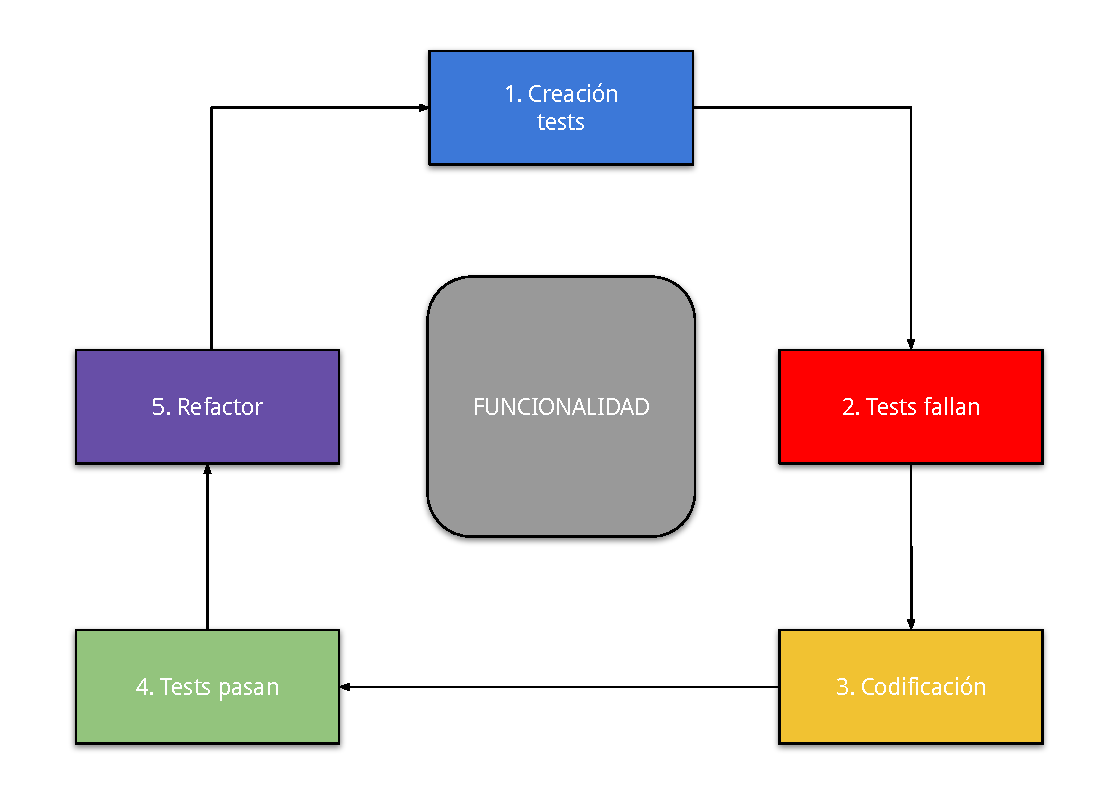
\includegraphics[scale=0.7]{images/tdd_diagram.pdf}
    \caption{Diagrama de flujo de la metodología TDD}
    \label{fig:tdd-diagram}
\end{figure}

La elección de la arquitectura \textit{Clean Architecture} en el proyecto es un aspecto que
facilita notablemente la implementación de la metodología en el proyecto, permitiendo
abstraer completamente los test para poder reutilizarlos incluso en otros casos de uso.

Las pautas de esta metodología sugieren un diagrama de flujo similar al de la \autoref{fig:tdd-diagram},
este flujo de estados se ha aplicado a todas las funcionalidades (\textit{features}) del
proyecto:

\begin{enumerate}
    \item De cara a integrar una nueva funcionalidad en el proyecto, se desarrolla una
    \textit{suite de tests}. La variedad de tipos de test es extensa, para el desarrollo
    de la aplicación se ha optado por tests \textit{unitarios} y \textit{de estado},
    con el fin de cubrir la mayor \textit{cobertura de código} posible.
    \item El siguiente paso consiste en ejecutar los tests, de forma evidente se obtiene 
    una serie de resultados fallidos ya que aún no se ha desarrollado la funcionalidad.
    \item En este momento se desarrolla la funcionalidad, dividida por las capas
    ya comentadas en el anterior capítulo.
    \item Conforme se va desarrollando la funcionalidad la ejecución de los tests
    van adquiriendo valores exitosos. De este modo, se asegura que la totalidad de las partes desarrolladas
    tengan los mínimos errores posibles.
    \item Una vez la ejecución de los tests de la funcionalidad tiene ausencia de errores 
    se procede a la \textit{refactorización} del código (desde cambios de nombres de variables
    hasta optimización de algoritmos desarrollados).
 \end{enumerate}